\section{System Design}\label{sec:design}
Fig.~\ref{fig:arch} shows the full ingestion-to-analytics design. Solid boxes inside the Spark job are implemented and measured in this paper. Dashed boxes are the AWS deployment around it, which we describe but did not run.

\begin{figure*}[t]
\centering
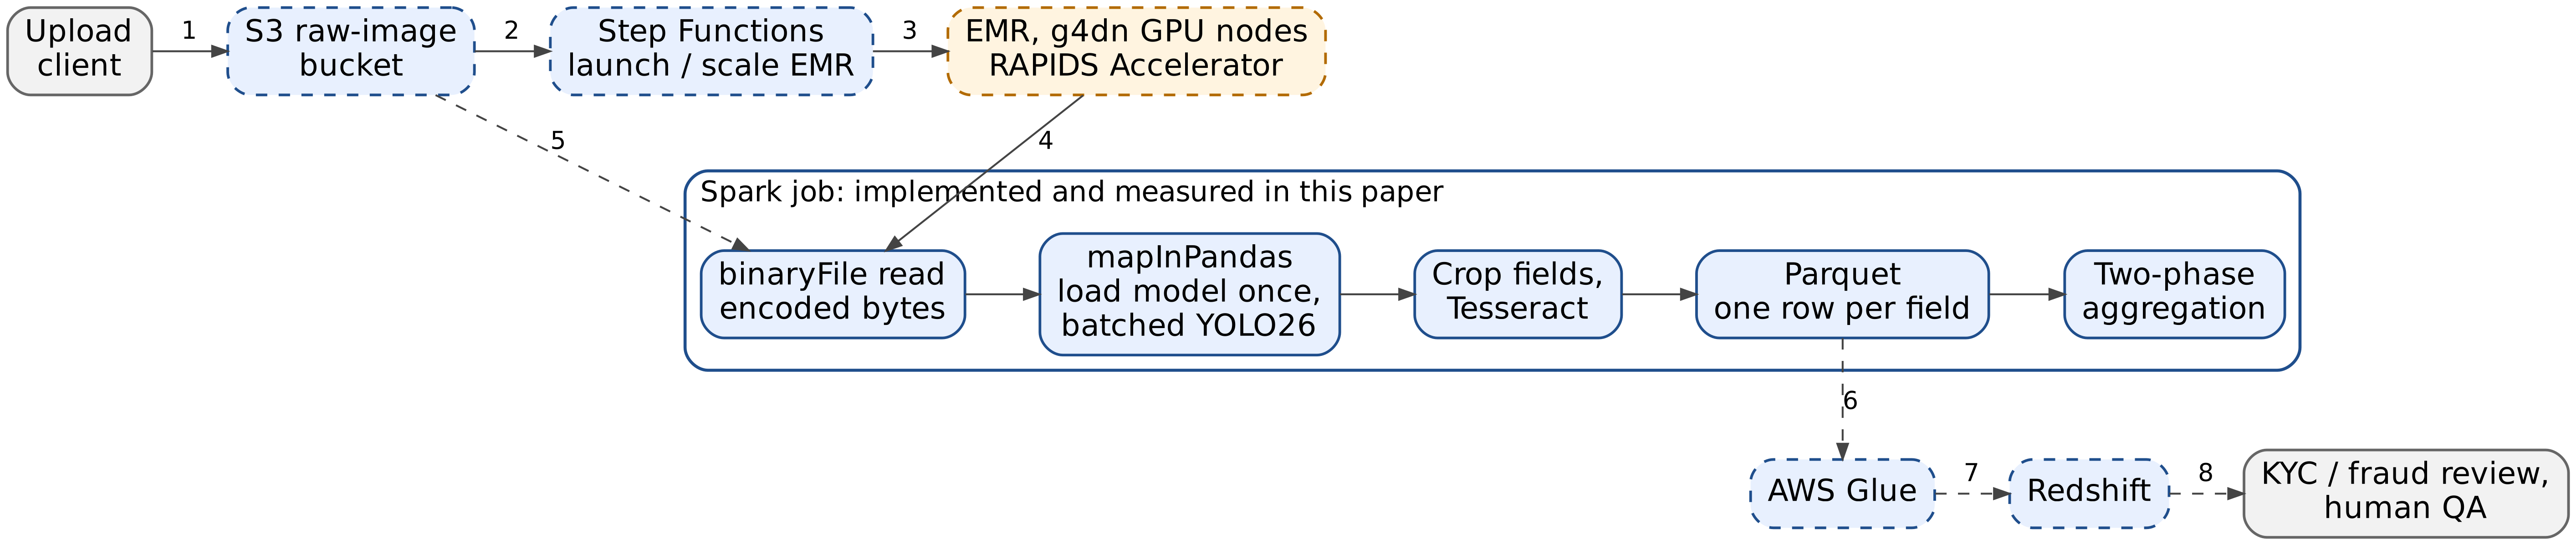
\includegraphics[width=0.98\textwidth]{figures/architecture.png}
\caption{Target architecture. The Spark job (solid) is implemented and measured here on a two-core CPU. Dashed components, including EMR with GPU nodes, Step Functions, Glue, and Redshift, are design only and were not exercised.}
\label{fig:arch}
\end{figure*}

\subsection{Spark job}
The job reads images with Spark\textquotesingle{}s \texttt{binaryFile} source, which returns the encoded file bytes unchanged. A \texttt{mapInPandas} function then runs once per partition. It loads the model once, decodes each Arrow batch of images, makes one batched detector call, crops every detected field from the original image, and runs Tesseract in single-line mode on each crop. Signature regions are detected but not read. Output is long format, one row per detected field, written as Parquet. A final step computes per-class mean confidence with a two-phase aggregation: each partition emits a partial sum and count, and Spark performs the final reduce. That step uses cuDF when RAPIDS is installed and pandas otherwise.

\subsection{Target deployment on AWS}
An upload to S3 raises an event, AWS Step Functions \cite{stepfunctions} launches or resizes an Amazon EMR \cite{emr} cluster, the Spark job runs, and structured output reaches Redshift through Glue. On a GPU cluster the detector would run on the device that Spark assigns to each task, using Spark\textquotesingle{}s custom resource scheduling \cite{spark_resources}, with one GPU per task slot. The pipeline module reads that device index from the task context and sets the corresponding Spark configuration when started with \texttt{--gpu}. We could not exercise this path, because no GPU was available, so it is untested.

\subsection{Where this design applies}
The design targets batch and micro-batch workloads, such as an overnight queue of scanned documents or a stream drained every few minutes. It does not target sub-second per-request latency. A cold EMR cluster adds a start-up cost that we did not measure and that no steady-state throughput figure includes. Interactive use would call for a warm cluster, EMR Serverless, or a plain model server in front of the same detector and OCR code.

\section{Implementation and Verified Defects}\label{sec:impl}
Table~\ref{tab:defects} lists the defects found in the first version of this pipeline. Each row records what was observed when the code was run, not what documentation predicts, except where marked as untested.

\begin{table*}[t]
\centering
\caption{Integration defects found by running the pipeline, and the fix applied in the released code.}
\label{tab:defects}
\small
\begin{tabular}{@{}p{0.2\textwidth}p{0.42\textwidth}p{0.32\textwidth}@{}}
\toprule
Defect & Observed behavior & Fix \\
\midrule
Spark \texttt{image} source fed to an image decoder & Returns decoded pixels, not file bytes. A 640 by 960 image gave 1{,}843{,}200 bytes against a 132{,}098 byte JPEG, and \texttt{imdecode} returned \texttt{None}. & Read with \texttt{binaryFile}, which returned bytes identical to the file. \\
Re-opening a path with \texttt{cv2.imread} & An \texttt{s3://} URI returns \texttt{None}. The path cannot be opened by OpenCV. & Decode the bytes Spark already read; never re-open the path. \\
\texttt{mapInPandas} on Spark 3.5.3 with JDK 21 & Fails in the JVM with \texttt{sun.misc.Unsafe or DirectByteBuffer.<init>(long, int) not available}, including with \texttt{--add-opens} and the Netty reflection flag. & Spark 4.0.1 on JDK 21 ran correctly. Spark 3.5 on JDK 17 is the documented alternative and was not tested. \\
Model constructed inside a row-wise UDF & The model loads once per row. Cost measured in Section~\ref{sec:results}. & Load once per partition inside \texttt{mapInPandas}. \\
Per-image Python loop around the model call & Inference is one image at a time. & One batched call per Arrow batch, with a dynamic-batch ONNX export. \\
Manual resize to 640 by 640 & Distorts non-square pages, and every box then needs mapping back to page coordinates. & Pass the original image. Ultralytics letterboxes internally and returns boxes in original pixels. \\
Hard-coded \texttt{device=0} with two concurrent GPU tasks & Two model copies can land on one device. \textit{Untested, no GPU available.} & Read the device from the task context and schedule one GPU per task. \\
cuDF used to count a substring in one JSON string & Too small an operation to benefit from a GPU, and the key it searched for did not match the output schema. & Per-partition partial sums and counts by class, reduced by Spark. \\
\bottomrule
\end{tabular}
\end{table*}

Listing~\ref{lst:partition} shows the core of the corrected pattern. The complete module, tests, and a one-command reproduction are in the released repository.\footnote{\repourl}

\begin{lstlisting}[language=Python,caption={Partition-level detection and OCR (abridged from \texttt{findoc/pipeline.py}).},label={lst:partition}]
def detect_partition(batches):
  device = _task_device()   # GPU from Spark, else CPU
  model = YOLO(SparkFiles.get(name))  # once
  for batch in batches:     # one Arrow batch
    imgs = [cv2.imdecode(
              np.frombuffer(bytes(raw), np.uint8),
              cv2.IMREAD_COLOR)
            for raw in batch["content"]]
    results = model(imgs, device=device)  # 1 call
    for path, im, res in zip(batch["path"],
                             imgs, results):
      for b in res.boxes:   # original pixels
        x1, y1, x2, y2 = map(int,
                             b.xyxy[0].tolist())
        text = pytesseract.image_to_string(
            gray(im[y1:y2, x1:x2]),
            config="--psm 7").strip()
        rows.append((path, cls(b), ..., text))
    yield pd.DataFrame(rows, columns=COLS)
\end{lstlisting}

\section{Experimental Setup}\label{sec:setup}
\textbf{Data.} A deterministic generator renders account forms at 960 by 640 pixels with five field classes: account number, date, amount, name, and signature. Layout, font, field order, noise, and blur vary per document. Every box and every text string is known exactly. The split is 240 training, 60 validation, and 60 test documents, with disjoint random seeds. The test split holds 300 fields, of which 240 carry text.

\textbf{Model.} YOLO26n fine-tuned from the COCO checkpoint for \valTrainEpochs{} epochs at 640 pixels, batch size 8, AdamW, on CPU, in about \valTrainMinutes{} minutes. We use the nano model because it is the one that trains on this hardware. The paper\textquotesingle{}s design uses the largest model on GPUs, and those results would differ.

\textbf{Hardware and software.} Two virtual CPU cores, 7 GB of memory, no GPU. Python 3.13, Spark 4.0.1, OpenJDK 21, Ultralytics 8.4, ONNX Runtime 1.29, Tesseract 5.3.4.

\textbf{Metrics.} A detection is correct if its class matches and its IoU with an unmatched ground-truth box is at least 0.5. We report precision and recall. End-to-end field accuracy is the share of text fields that are both localized and read with an exact string match after whitespace is removed. The baseline is Tesseract run on the full page. We count a field as captured if its exact string appears anywhere in the page text. That rule is lenient, because the baseline is never required to say which field a string belongs to, so it is an upper bound on what page-level OCR delivers and is not a like-for-like extractor.

\textbf{Inference-pattern timing.} The same fine-tuned model scores \valPatDocs{} test documents on two partitions in three configurations: a row-wise UDF that builds the model on every call, and \texttt{mapInPandas} with Arrow batch sizes 1 and 16. Detection only, no OCR, so the comparison isolates the pattern. Each configuration has one discarded warm-up run and \valPatRepeats{} timed runs.

\textbf{Limits of the design.} There is one training seed, and the test split is 60 documents, so intervals are wide and we report Wilson 95 percent intervals where they matter. The dataset is synthetic, clean, and easy by comparison with scanned documents, so absolute accuracy here says little about real documents.
